\documentclass[12pt]{article}
\usepackage[scaled]{helvet}
\renewcommand\familydefault{\sfdefault} 
\usepackage[T1]{fontenc}

\usepackage[english]{babel}
\usepackage[utf8]{inputenc}
\usepackage{amsmath,amssymb}
\usepackage{parskip}
\usepackage{graphicx}
\usepackage{listings}

\title{\textbf{Practical 1: Projectile Motion}}
\author{Babis Koniaris}
\date{}

\begin{document}
\maketitle

\begin{center}
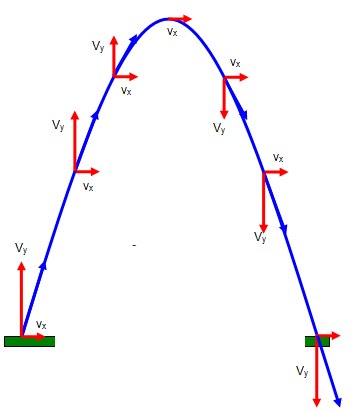
\includegraphics[scale=1]{p1-teaser.png}
\end{center}
\pagebreak

\section*{Introduction}

The goals of this first practical are to:

\begin{itemize}
\item Give you an opportunity to become familiar with the code that is provided to you.
\item Write simple (time-based) animations
\item Use the equations of motion to implement physically-plausible animations
\end{itemize}

\subsection*{Working with the provided code}

The code is provided as a CMake project. CMake is used here to create visual studio projects from a text description. Read the instructions in the main repository README carefully, as CMake might seem weird and difficult, but once you set it up, you can (re-)generate visual studio projects very quickly.

We are using a few libraries: GLEW, GLFW, glm and tinyobjloader. GLEW is used for OpenGL initialisation, GLFW is used for the window creation and input handling, glm is a very useful mathematics library (vector math, matrix math, quaternion math, and datatypes) and tinyobjloader is used to load simple 3D models.

\section*{Development approach}

The focus of this module is the development of physics-based simulations, not graphics programming or game engine development. Therefore it would seem reasonable to provide you with a game engine that contains everything you need except the physics part. However, such engines contain several things not useful for this module, and to avoid distractions, we are going to use a basic low-level real-time application framework that we can adapt to our specific needs. These needs will evolve every week, so our architecture will be relatively dynamic.

\section*{Code in the repository}

The repository contains four projects. 

\begin{itemize}
\item The first project (01\_particle\_animation) is a very simple framework to make you familiarised with GLFW, which acts as the hook to the display and input. It's going to be used only in the first week, so that you can have a cursory look to what some basic GLFW code looks like (including setting up a basic shader and rendering). 
\item The second project (02\_particles\_framework) is a more structured framework which will form the basis of all your practical work and coursework. Here we're going to use classes to represent the application, the physics engine, static objects such as ground and the individual particles that need to be simulated. 
\item The third and fourth projects contain minor additions to this framework, to take into account forces and rigid bodies respectively
\end{itemize}

\section*{Code for first week}

All code is in four files: Camera.h, Mesh.h, Shader.h and 01\_particle\_animation.cpp. The first three are self-explanatory, and contain definitions for the camera, mesh and shaders. What's most important this week is the file 01\_particle\_animation.cpp. Let's see what it contains, before we proceed with the tasks:

\subsection*{main}

At the end of the file, we find the definition for the main() function, which is the entry point of the program. You can see the structure is very simple: we start with some window/OpenGL initialisation code (initRender()), then proceed with initialisation of some variables that require a valid window and OpenGL context (shader and mesh), and then we set up two objects: a particle and the ground. We then initialise some time-keeping variables and proceed in the game loop: 

\begin{center}
\texttt{while (!glfwWindowShouldClose(window)) \{...\}}
\end{center}

Inside the loop we update the time-keeping variables, we handle input, update the camera, animate our objects and display everything. This is where you'll run your experiments this week to animate the particle(s). If we exit the loop, we destroy the window and exit the application.

The positions, velocities and accelerations are all 3D vectors, using the GLM library (glm::vec3).

\section*{Manipulating the position and orientation of objects}

To animate objects, we eventually have to manipulate matrices, but thankfully we don't do that directly. There is a chain of events that needs to happen, to ease this process. Each object that needs to be animated is represented by a mesh, which is a collection of vertices. To place a mesh in the world, we use a 4x4 homogeneous matrix that contains orientation, scaling and translation. So, everytime we move an object, we apply a translation operation to its matrix. When we rotate an object, we change the orientation (and sometimes the translation). This week, the ```Object``` class stores the ingredients for the homogeneous matrix (orientation, translation and scaling) and we only have to give high level instructions (rotate by that much) and the code handles the conversion to the homogeneous matrix (ModelMatrix() function). So, feel free to experiment with the functions of the Object class to rotate, scale and move the objects.

\section*{Tasks}

For this week, first get familiarised with the code (we'll be moving to a restructuring of this code next week though), and try to animate the particles! The particle shape for this week is a simple tetrahedron, and you'll get more choices from next week onwards. 

\subsection*{Task 1: Particle movement using SetPosition()}

Show the same particle movement as the default one (constant speed, downwards) by using the SetPosition() method instead of the Translate() method

\subsection*{Task 2: Particle acceleration}

Show the particle accelerating downwards, under the force of gravity

\subsection*{Task 3: Particle oscillation}

Make the particle oscillate around the ground, between y == -5 and y == +5. You can use trigonometric functions, such as sine and cosine

\subsection*{Task 4: Particle trajectory}

Animate a particle based on its initial position, velocity and acceleration (the latter being constant). Here you are supposed to apply the equations of motion. Choose what you want for the initial position and velocity and use glm::vec3(0,-9.81,0) for acceleration.

\subsection*{Task 5: Collision}

Make the particle bounce by adding a collision test with the ground plane. Here's additional information to clarify the task:

\begin{itemize}
\item Assume that the ground plane is infinitely large, so testing for collision with the plane equates to testing that a particle is at the height of the plane (or close to it, or below). 
\item To implement a bounce, consider what needs to happen to the velocity when a collision is detected. Although we haven't covered the concept of energy loss/conservation, you can deal with the problem intuitively and consider different behaviours: a particle could lose energy on impact and see its velocity decrease, or it could bounce forever without ever stopping. You can also make it bounce with increased velocity any time there is contact with the plane. The first behaviour seems like a natural one for most physical surfaces, while the last one would make sense if the ground floor represents a pinball kicker.
\item Add whatever variables you need.
\end{itemize}

\subsection*{Task 6: Many particles}

Same as task 5, but for a collection of particles. If you can get one particle to bounce around, you will undoubtedly want to see how many you can animate. To make the animation interesting, give them all different (random) initial velocities. There are two interesting aspects to this task: 

\begin{itemize}
\item Code change required to make it work, including data structures needed to hold information about the particles
\item Optimisation: how many particles can you animate concurrently? 1,000, 10,000, 1 million? I’m not asking you to make any change to the code that will increase this number (I'm not stopping you either!), but I’d like you to reflect on what could be done to improve performance.
\end{itemize}

\subsection*{Deliverables}

No deliverables this week. From next week onwards, some of the practical work that you do will be part of your marked coursework.

\end{document}
